% !Mode:: "TeX:UTF-8"
% !Mode:: "TeX:UTF-8"
\newcommand{\thepage}{} % to silence a hyperref warning about pdfpagelabels
\RequirePackage[]{silence}
\WarningsOff[hyperref]
\PassOptionsToPackage{log-declarations=false}{xparse}
%\RequirePackage[l2tabu, orthodox]{nag}
\RequirePackage{luatex85} % to make \pdf...= commands work with LuaTeX
\documentclass[aspectratio=169,t]{beamer}
\usepackage{ifthen}
\usepackage[T1]{fontenc}
\usepackage{iftex}
\ifLuaTeX
 \usepackage{fontspec}
 \setmainfont[Ligatures=TeX]{Source Sans Pro}
\else
 \usepackage[utf8]{inputenc}
\fi
\usepackage{german}
\usepackage{newunicodechar}
\newunicodechar{€}{\texteuro}
\newunicodechar{ß}{\ss}
\renewcommand{\SS}{\iffontchar\font"1E9E \symbol{"1E9E}\else SS\fi}
\usepackage{ellipsis}
\usepackage{microtype}
\usepackage{listings}
\usepackage{sourcecodepro}
\lstset{language=Python, basicstyle=\ttfamily}
\usepackage{amsfonts}
\usepackage{amssymb}
\usepackage{amsthm}
\usepackage{fancyhdr}
\usepackage{graphicx}

\newtheorem{proposition}[theorem]{Proposition}

\DeclareMathOperator*{\argmax}{argmax}
\DeclareMathOperator{\supp}{supp}
\newcommand{\E}{\ensuremath{\mathbb{E}}}
\newcommand{\V}{\ensuremath{\mathbb{V}}}

\setbeamercolor{emph}{fg=purple}
\renewcommand<>{\emph}[1]{%
  {\usebeamercolor[fg]{emph}\only#2{\itshape}#1}%
}



\hypersetup{draft=false,colorlinks=false,pdfpagemode=UseOutlines,plainpages=false,
            breaklinks=true,bookmarksnumbered=true,pdfborder=0 0 0,
            pdftitle={Data Science SoSe 2026 HHU},
            pdfauthor={Konrad Voelkel},
            pdfsubject={data science}}

%\documentclass[aspectratio=169,t]{beamer}
\usetheme{hhubeamer} % put the hhu-beamer-theme in /usr/share/texmf/tex/latex/beamer/themes/

% -------------------- Code listings config --------------------
% Define custom colors for syntax highlighting
\definecolor{codegreen}{rgb}{0,0.6,0}
\definecolor{codegray}{rgb}{0.5,0.5,0.5}
\definecolor{codepurple}{rgb}{0.58,0,0.82}
\definecolor{backcolour}{rgb}{0.96,0.96,0.94} % Very light gray/beige
% Configure the listings package
\lstset{
    language=Python,
    backgroundcolor=\color{backcolour},   
    commentstyle=\color{codegreen}\itshape,
    keywordstyle=\color{blue}\bfseries,
    numberstyle=\tiny\color{codegray},
    stringstyle=\color{codepurple},
    basicstyle=\ttfamily\footnotesize, % Use a monospaced font
    breakatwhitespace=false,         
    breaklines=true,      
             % Enable automatic line breaking
    captionpos=b,                      % Caption at the bottom
    keepspaces=true,                 
    numbers=left,                      % Line numbers on the left
    numbersep=10pt,                    % Distance of line numbers from the code
    showspaces=false,                
    showstringspaces=false,            % Don't show weird underscores in strings
    showtabs=false,                  
    tabsize=4,
    frame=single,                      % Add a subtle border around the code
    rulecolor=\color{black!20},        % Border color
  }

\event[]{}
\author[Sommersemester 2026]{Dr. Konrad Völkel, Sommersemester 2026}

%\title{Data Science, VL 1}
%\date{16.04.2026}


%%% Local Variables:
%%% mode: latex
%%% TeX-master: t
%%% End:


\title{Data Science, VL 8}
\subtitle{Die Gaußsche Normalverteilung}
\date{19.05.2026}


\begin{document}

\begin{frame}
  \titlepage
\end{frame}

\section{Approximation der Binomialverteilung}

\begin{frame}
  \frametitle{Summen von Bernoulli-Variablen}
  \begin{itemize}[<+->]
  \item Betrachten wir eine Folge von Bernoulli-verteilten Zufallsvariablen $X_i$ mit gleichem Parameter $p$.
  \item Die Summe $S_n := \sum_{i=1}^n X_i$ über die ersten $n$ Variablen ist \alert{binomialverteilt}: $S_n \sim Bin(n,p)$.
  \item Die Wahrscheinlichkeitsfunktion (pmf) von $S_n$ lautet bekanntlich:
  \[ p(k) = P(S_n = k) = \binom{n}{k}p^k(1-p)^{n-k} \]
  \item Für große $n$ nähert sich die Form des Histogramms stets einer Glockenkurve an. 
  \item Da Binomialkoeffizienten für große $n$ schwer exakt zu berechnen sind (Fakultäten wachsen extrem schnell), sucht man nach einer \alert{stetigen Approximation}.
  \end{itemize}
\end{frame}

\begin{frame}[fragile]
  \frametitle{Plot eines binomialverteilten Samples}
\begin{lstlisting}[language=Python]
import numpy as np
from scipy.stats import binom, norm
from matplotlib import pyplot as plt
np.random.seed(123123)
binom_samples = binom.rvs(n=100,
                          p=0.4,
                          size=100000)
plt.hist(binom_samples, bins=40, density=True)
plt.xlabel("x binomialverteilt")
plt.ylabel("Dichte")
plt.show()
\end{lstlisting}
\end{frame}

\begin{frame}

\includegraphics[width=0.7\textwidth]{figures/binomial-histogram.png}
\end{frame}

\begin{frame}
  \frametitle{Satz von de Moivre-Laplace}
  \begin{block}{Stirling-Formel zur Approximation}
    \[ n! \approx \sqrt{2\pi n} {\left(\frac{n}{e}\right)}^n \]
  \end{block}
  \pause
  Damit lässt sich für die Binomialverteilung zeigen:
  \[ P(S_n = k) \sim \frac{1}{\sqrt{np(1-p)}} \frac{1}{\sqrt{2\pi}} e^{-\frac{x_n^2}{2}} \quad \text{ für } n \to \infty \]
  wobei $x_n = \frac{k-np}{\sqrt{np(1-p)}}$ eingesetzt wird.\pause
  
  \vspace{0.5cm}
  Das Symbol $\sim$ bedeutet asymptotische Gleichheit (der Quotient konvergiert gegen $1$). Die Funktion $e^{-x^2/2}$ spielt hier also die zentrale Rolle.
\end{frame}

\begin{frame}
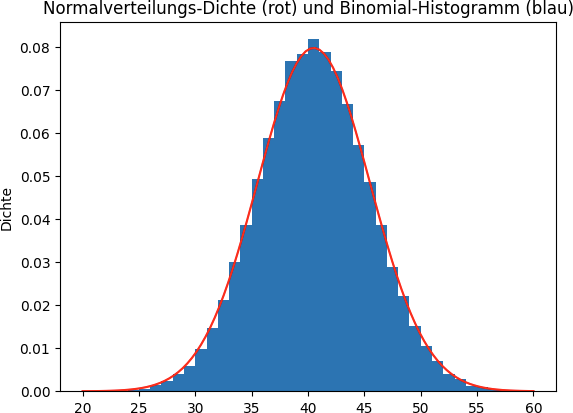
\includegraphics[width=0.7\textwidth]{figures/binomial-histogram-normal.png}
\end{frame}

\section{Ein Integral}

\begin{frame}
  \frametitle{Das Gaußsche Integral}
  Um aus $e^{-x^2/2}$ eine Wahrscheinlichkeitsdichte zu machen, muss das Integral über $\mathbb{R}$ gleich $1$ sein. Wir betrachten ein allgemeineres Integral:
  \pause
  \begin{lemma}
    Sei $v \in \mathbb{R}$ und $v > 0$. Dann gilt
    \[ \int_{-\infty}^\infty e^{-\frac{x^2}{2v}} dx = \sqrt{2\pi v}. \]
  \end{lemma}
\end{frame}

\begin{frame}
  \frametitle{Beweis des Gaußschen Integrals (1/2)}
  \begin{proof}
    Wir quadrieren das Integral und transformieren es in Polarkoordinaten:
    \begin{align*}
      {\left( \int_{-\infty}^\infty e^{-\frac{x^2}{2v}} dx \right)}^2 
      &= \int_{-\infty}^\infty e^{-\frac{x^2}{2v}} dx \int_{-\infty}^\infty e^{-\frac{y^2}{2v}} dy \\
      \uncover<2->{&= \int_{-\infty}^\infty \int_{-\infty}^\infty e^{-\frac{x^2+y^2}{2v}} dx dy = \int_{\mathbb{R}^2} e^{-\frac{x^2+y^2}{2v}} d(x,y) \\}
      \uncover<3->{&= \int_{0}^\infty \int_{0}^{2\pi} r e^{-\frac{r^2}{2v}} d\phi dr = \int_{0}^\infty r e^{-\frac{r^2}{2v}} [\phi]_0^{2\pi} dr \\}
      \uncover<4->{&= 2\pi \int_{0}^\infty r e^{-\frac{r^2}{2v}} dr \\}
    \end{align*}
  \end{proof}
\end{frame}

\begin{frame}
  \frametitle{Beweis des Gaußschen Integrals (2/2)}
  \begin{proof}
    Wir quadrieren das Integral und transformieren es in Polarkoordinaten:
    \begin{align*}
      \uncover<0->{&= 2\pi \int_{0}^\infty r e^{-\frac{r^2}{2v}} dr \\}
      \uncover<1->{&= 2\pi v \int_{-\infty}^{0} e^u du \quad \text{(Substitution } u = -r^2/(2v) \text{)} \\}
      \uncover<2->{&= 2\pi v [e^u]_{-\infty}^{0} = 2\pi v.}
    \end{align*}
    \uncover<3->{Wurzelziehen liefert die Behauptung.\qedhere}
  \end{proof}
\end{frame}

\section{Die Normalverteilung}

\begin{frame}
  \frametitle{Die eindimensionale Normalverteilung}
  \begin{definition}
    Seien $\mu,\sigma \in \mathbb{R}$ mit $\sigma > 0$. Dann heißt die Verteilung mit der Dichtefunktion
    \[ \phi(x) = \frac{1}{\sigma\sqrt{2\pi}} e^{-\frac{(x-\mu)^2}{2\sigma^2}} \]
    \alert{Normalverteilung}.

    Für eine reelle Zufallsvariable $X$ mit dieser Verteilung schreiben wir $X \sim \mathcal{N}(\mu,\sigma^2)$.
  \end{definition}
  \pause
  \begin{definition}
    Eine Zufallsvariable mit $X \sim \mathcal{N}(0,1)$ heißt \alert{standardnormalverteilt}.
  \end{definition}
\end{frame}


\begin{frame}
  \frametitle{Erwartungswert und Varianz}
  \uncover<0-1>{
  \begin{proposition}
    Wenn $X \sim \mathcal{N}(\mu,\sigma^2)$, so ist $\E(X) = \mu$ und $\V(X) = \sigma^2$.
  \end{proposition}
  }
  \pause
  \vspace{-2.5cm}
  \begin{proof}[Beweis-Skizze für den Erwartungswert]
    \begin{align*}
      \E(X) &= \frac{1}{\sigma\sqrt{2\pi}} \int_{-\infty}^{\infty} x e^{-\frac{(x-\mu)^2}{2\sigma^2}} dx \\
      \uncover<3->{&= \frac{1}{\sigma\sqrt{2\pi}} \int_{-\infty}^{\infty} (x+\mu) e^{-\frac{x^2}{2\sigma^2}} dx \quad \text{(Substitution } x \mapsto x+\mu \text{)} \\}
      \uncover<4->{&= \underbrace{\frac{1}{\sigma\sqrt{2\pi}} \int_{-\infty}^{\infty} x e^{-\frac{x^2}{2\sigma^2}} dx}_{= 0 \text{ (aus Symmetrie)}} + \mu \underbrace{\frac{1}{\sigma\sqrt{2\pi}} \int_{-\infty}^{\infty} e^{-\frac{x^2}{2\sigma^2}} dx}_{= 1 \text{ (Dichte)}} \\}
      \uncover<5->{&= \mu.}
    \end{align*}
  \end{proof}
\end{frame}

\begin{frame}
  \frametitle{Eigenschaften der Normalverteilung}
  \begin{proposition}
    Wenn $X \sim \mathcal{N}(\mu,\sigma^2)$, so ist $\frac{X - \mu}{\sigma} \sim \mathcal{N}(0,1)$.
  \end{proposition}
  \pause\medskip
  Es ist offensichtlich, dass $\E\left(\frac{X-\mu}{\sigma}\right) = 0$ und $\V\left(\frac{X-\mu}{\sigma}\right) = 1$.

  Die Normalverteiltheit bleibt unter linearen Transformationen erhalten.
  
  \pause\vspace{0.5cm}
  \begin{proposition}
    Wenn $X \sim \mathcal{N}(\mu_1,\sigma_1^2)$ und $Y \sim \mathcal{N}(\mu_2,\sigma_2^2)$ unabhängig sind, so ist 
    \[ X+Y \sim \mathcal{N}(\mu_1 + \mu_2, \sigma_1^2 + \sigma_2^2). \]
  \end{proposition}
\end{frame}

\begin{frame}
  \frametitle{Maximale Entropie}
  \begin{theorem}
    Unter allen stetigen Verteilungen reeller Zufallsvariablen mit Träger ganz $\mathbb{R}$ und festem Erwartungswert $\mu$ und Varianz $\sigma^2$ ist die Normalverteilung diejenige mit der \alert{maximalen Entropie}.
  \end{theorem}
  \pause
  \vspace{0.5cm}
  \textbf{Take-Home-Message:} Wenn über eine Verteilung (außer Träger, Erwartungswert und Varianz) nichts bekannt ist, dann ist die Normalverteilung die unvoreingenommenste und vernünftigste Annahme.
\end{frame}

\begin{frame}
  \frametitle{Ausblick: Maximale Entropie bei anderem Träger}
  Je nach Träger (support) und den bekannten Parametern ergeben sich andere Verteilungen als \alert{unvoreingenommenste Annahme} (Maximale Entropie):
  
  \vspace{0.3cm}
  \begin{itemize}[<+->]
    \item \textbf{Träger $[a,b]$} (endliches Intervall), keine weiteren Parameter bekannt:\\
    $\Rightarrow$ \alert{Stetige Gleichverteilung} $\frac{1}{b-a}$
    
    \vspace{0.2cm}
    \item \textbf{Diskreter Träger $\{1, \dots, n\}$}, keine weiteren Parameter bekannt:\\
    $\Rightarrow$ \alert{Diskrete Gleichverteilung} $\frac{1}{n}$
    
    \vspace{0.2cm}
    \item \textbf{Träger $[0, \infty)$} (nur positive Werte), fester Erwartungswert $\mu$ bekannt:\\
    $\Rightarrow$ \alert{Exponentialverteilung} $\lambda e^{-\lambda x}$ für $x\geq 0$, wobei $\lambda = \frac{1}{\mu}$.
    
    \vspace{0.2cm}
    \item \textbf{Träger $[a,b]$} (endliches Intervall), feste Varianz $\sigma^2$ bekannt:\\
    $\Rightarrow$ \alert{Gestutzte Normalverteilung}
  \end{itemize}
\end{frame}

\section{Der zentrale Grenzwertsatz}

\begin{frame}
  \frametitle{Der zentrale Grenzwertsatz (CLT)}
  \begin{theorem}[Zentraler Grenzwertsatz]
    Wenn $(X_i)_{i \in \mathbb{N}}$ eine Folge von unabhängig und identisch verteilten (iid) Zufallsvariablen mit $\E(X_i)=0$ und $\V(X_i)=\sigma^2$ ist, dann gilt für die reskalierte Summe $S_N := \frac{1}{\sigma\sqrt{N}} \sum_{i=1}^N X_i$ die Konvergenz in Verteilung:
    \[ S_N \xrightarrow{N \to \infty} \mathcal{N}(0,1) \]
  \end{theorem}
  \pause
  \begin{itemize}
    \item \textbf{Bedeutung in der Praxis:} Die Summe vieler kleiner, unabhängiger Fehlereinflüsse ist am Ende oft annähernd normalverteilt.
    \item Beispiele: Messfehler bei GPS-Systemen, Abweichungen in der industriellen Fertigung.
  \end{itemize}
\end{frame}

\begin{frame}
  \frametitle{Konvergenzgeschwindigkeit (Berry-Esseen)}
  Wie schnell konvergiert die Verteilung gegen die Normalverteilung?
  \pause
  \begin{theorem}
    Es existiert eine Konstante $C > 0,4409$ mit der Eigenschaft:
    Wenn $X_i$ iid sind mit $\E(X_i) = 0$, $\V(X_i) = \sigma^2$ und $\E|X_i^3| = \rho < \infty$, so gilt für die kumulative Verteilungsfunktion $F_N$ von $\frac{1}{\sigma\sqrt{N}} \sum_{i=1}^N X_i$ und die cdf $\Phi$ von $\mathcal{N}(0,1)$:
    \[ \sup_{x \in \mathbb{R}} \left| F_N(x) - \Phi(x) \right| \leq \frac{C\rho}{\sigma^3 \sqrt{N}}. \]
  \end{theorem}
  \pause
  \vspace{0.3cm}
  Damit lässt sich für bekannte Parameter abschätzen, wie groß $N$ sein muss, um eine gewünschte Genauigkeit für die Normalapproximation zu erzielen.
\end{frame}

\begin{frame}
  \frametitle{Praxisbeispiel: Der \glqq $N \ge 30$\grqq-Mythos}
  \textbf{Mythos:} \glqq Bei Stichproben ab $N=30$ darf man eine Normalverteilung annehmen.\grqq
  \pause
  
  \vspace{0.3cm}
  Warum das (gerade bei medizinischen Studien mit binären Daten) \alert{falsch} ist:
  \begin{itemize}[<+->]
    \item Bei binären Merkmalen (z.\,B. Nebenwirkung ja/nein) liegt eine Bernoulli-Verteilung vor.
    \item Wenn das Ereignis selten ist (z.\,B. $p=0.01$), ist diese Verteilung extrem schief.
    \item \textbf{Berry-Esseen zeigt:} Der Approximationsfehler hängt maßgeblich vom dritten Moment (der Schiefe) ab! Ist $\E|X_i^3|$ im Verhältnis zu $\sigma^3$ groß, reicht $n=30$ bei Weitem nicht aus, um den Fehler klein zu halten.
  \end{itemize}
\end{frame}

\begin{frame}
  \frametitle{Praxisbeispiel: Faustregel}
  \begin{block}{Die korrekte Faustregel für binäre Daten}
    Eine Normalapproximation ist erst gerechtfertigt, wenn die erwartete absolute Häufigkeit für beide Ausprägungen groß genug ist (\alert{Laplace-Bedingung}):
    \[ N \cdot p \ge 10 \quad \text{und} \quad N \cdot (1-p) \ge 10 \]
    Bei einer seltenen Krankheit mit $p=0.01$ braucht man also mindestens $N=1000$ Probanden!
  \end{block}
\end{frame}

\begin{frame}[separator]
  \frametitle{Vielen Dank für Ihre Aufmerksamkeit!}
\end{frame}

\end{document}

%%% Local Variables:
%%% mode: latex
%%% TeX-master: t
%%% End:
